% !Mode:: "TeX:UTF-8"
\chapter{可见光多波段OFDM系统的信道估计}
\section{引言}
所谓信道估计,就是在接收端估计出信道状态信息(Channel State Information,CSI),为下一步地解调做准备,也是自适应传输技术的基础。无线通信一个重要的特征就是发射端到接收端之间的路径比较复杂,不像有线通信那样是固定且可预知的,所以信道估计技术在无线通信领域格外重要,特别是在OFDM 等需要相干检测的系统中。本章将着重介绍信道估计技术,首先介绍传统射频通信中OFDM 系统的信道估计方法,然后具体到可见光通信系统中的信道估计问题,再将结合实际系统设计,讨论信道的非线性问题,最后将研究多色可见光通信系统中各波段之间串扰的估计。
\section{OFDM信道估计常用方法}
信道估计总体可以分为两大类,盲信道估计和基于导频的信道估计。盲信道不需要额外的导频或者训练序列,因此频率利用率高;但是它的缺点是计算量大、算法复杂,而且精度低、收敛速度缓慢,难以用于移动通信环境
\cite{石钧2012ofdm}。基于导频的信道估计原理是在发射端插入专门用于信道估计的导频或者训练序列,并且这些序列对于接收端也是已知的,接收端根据接收到的经过了信道后的导频序列与原导频序列之间的关系,估计出信道冲击响应(Channel Impulse Response,CIR)。这类信道估计方法因为要插入导频序列会稍微降低整个系统的传输速率,但是其估计实现复杂度低、估计精度高,在实际工程中大都采用这种方法。本节也主要讨论基于导频的信道估计算法。
\begin{figure}[htbp]
    \centering
    \subfloat[块状导频放置方式]{
        \label{fig:BlockTypePilot}
        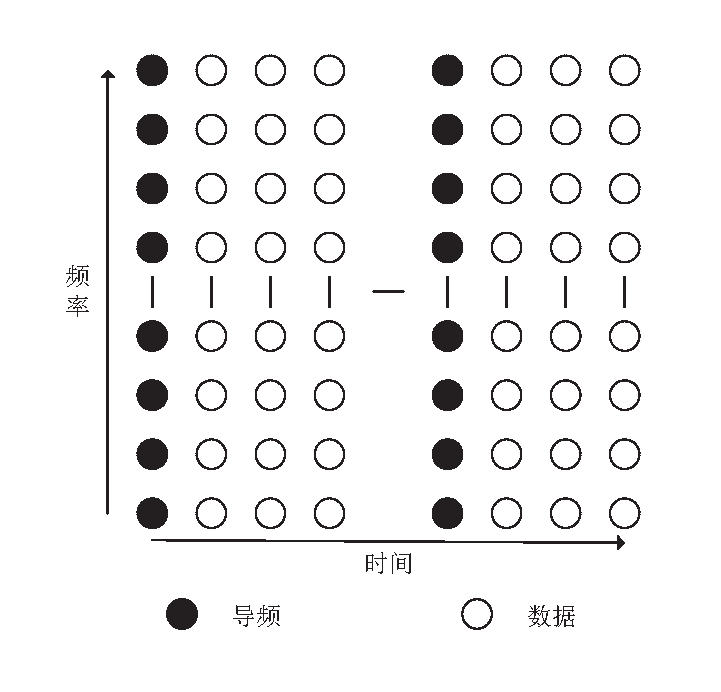
\includegraphics[width = 0.5\textwidth]{figures/chapter-3/BlockTypePilot.eps}
    }
    \subfloat[梳状导频放置方式]{
    	\label{fig:CombTypePilot}
        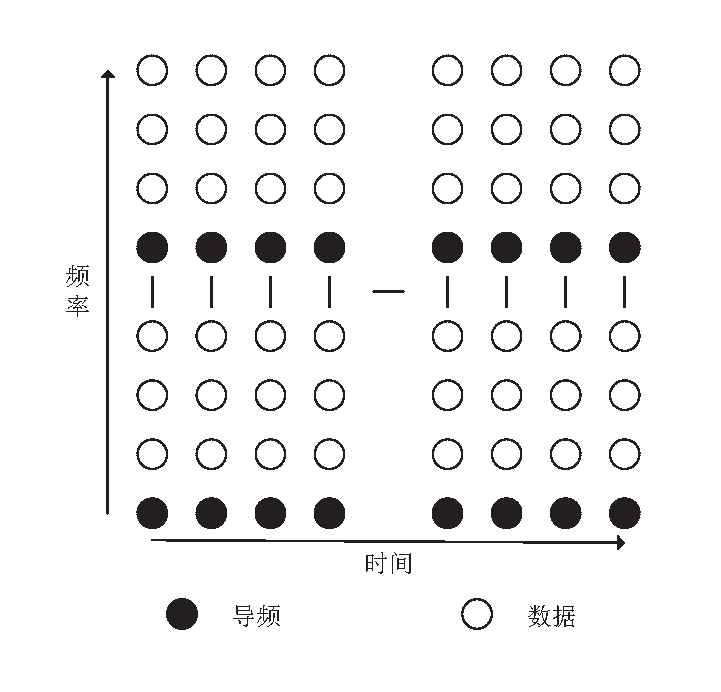
\includegraphics[width = 0.5\textwidth]{figures/chapter-3/CombTypePilot.eps}
    }
    \caption{导频放置方式}
    \label{fig:PilotAllocation}
\end{figure}
对于基于导频的信道估计而言,研究人员对其导频放置方式也进行了深入的研究,如\autoref{fig:PilotAllocation}所示,常见的有块状和梳状两种放置方式。

块状导频放置方式见图\ref{fig:BlockTypePilot},它的导频序列连续放置在一个OFDM符号上,但是在时间上不是连续的,也就是说要隔若干个OFDM符号才放置一个导频序列。在工程实现中,更常见的一种情况是导频序列即用于信道估计,又用于同步,这样一般是一帧放置一个导频符号。块状导频放置方式的优点是结构简单,计算复杂度低,但是因为要隔一段时间才估计一次信道,所以块状导频放置方式一般用于信道时变比较缓慢的信道。

梳状导频放置方式如图\ref{fig:CombTypePilot}所示,在每个OFDM符号上,它只选择在特定的子载波上放置导频序列,而其他子载波上放置数据符号,并且每个OFDM符号的结构都是如此。它的工作原理是先估计出放置了导频的子载波处的信道响应,然后根据这些信道响应通过插值的方式得到那些放置了数据符号的子载波处的信道响应。它的优点是每个符号都会估计信道,能够应对快速时变的信道,但是它要使用插值计算,所以复杂度比较高,并且估计准确度也较低。
\section{可见光各波段之间串扰估计}
\section{本章小结}
